% An augmenting path (generated by figs_c1ch06.py).
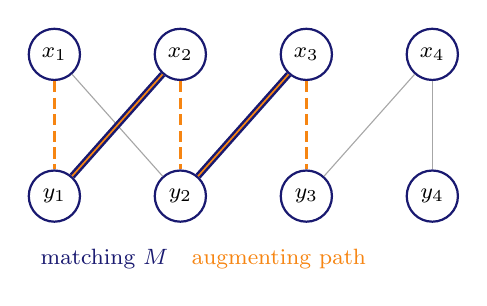
\begin{tikzpicture}[x=1cm,y=1cm,v/.style={circle,draw=MidnightBlue,thick,fill=white,inner sep=1.5pt,minimum size=6.5mm,font=\footnotesize},e/.style={gray!70},m/.style={line width=2.4pt,MidnightBlue},p/.style={line width=1.1pt,BurntOrange,dash pattern=on 4pt off 2pt}]
\node[v] (x1) at (0.0,1.8) {$x_1$};
\node[v] (x2) at (1.6,1.8) {$x_2$};
\node[v] (x3) at (3.2,1.8) {$x_3$};
\node[v] (x4) at (4.800000000000001,1.8) {$x_4$};
\node[v] (y1) at (0.0,0) {$y_1$};
\node[v] (y2) at (1.6,0) {$y_2$};
\node[v] (y3) at (3.2,0) {$y_3$};
\node[v] (y4) at (4.800000000000001,0) {$y_4$};
\draw[e] (x1) -- (y2); \draw[e] (x4) -- (y3); \draw[e] (x4) -- (y4);
\draw[m] (x2) -- (y1); \draw[m] (x3) -- (y2);
\draw[p] (x1) -- (y1); \draw[p] (x2) -- (y2); \draw[p] (x3) -- (y3);
\draw[p,line width=0.6pt,dash pattern=] (x2) -- (y1); \draw[p,line width=0.6pt,dash pattern=] (x3) -- (y2);
\node[font=\footnotesize,anchor=west] at (-0.3,-0.8) {\textcolor{MidnightBlue}{matching $M$}\quad \textcolor{BurntOrange}{augmenting path}};
\end{tikzpicture}
